% Figure 3: VRA Compliance Analysis (3-panel figure)
% Requires data from papers 3, 4, 6

\begin{figure*}[t]
\centering

% Panel A: Bar chart of MM districts (enacted vs. algorithmic)
\begin{subfigure}[b]{0.32\textwidth}
\centering
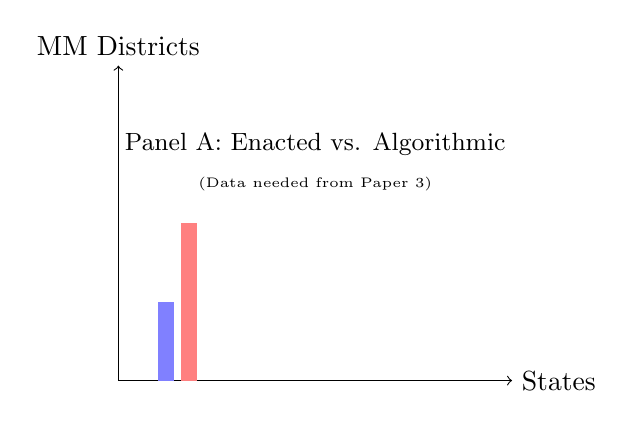
\begin{tikzpicture}[scale=0.5]
% Placeholder - needs actual data
\draw[->] (0,0) -- (0,8) node[above] {MM Districts};
\draw[->] (0,0) -- (10,0) node[right] {States};
% Example bars for illustration
\fill[blue!50] (1,0) rectangle (1.4,2);
\fill[red!50] (1.6,0) rectangle (2,4);
\node at (5,6) {\small Panel A: Enacted vs. Algorithmic};
\node at (5,5) {\tiny (Data needed from Paper 3)};
\end{tikzpicture}
\caption{MM district counts by state}
\end{subfigure}
\hfill
% Panel B: 42% threshold scatter plot
\begin{subfigure}[b]{0.32\textwidth}
\centering
\begin{tikzpicture}[scale=0.5]
% Placeholder - needs actual data
\draw[->] (0,0) -- (10,0) node[right] {State Minority \%};
\draw[->] (0,0) -- (0,8) node[above] {MM Success};
% Threshold line
\draw[thick, red, dashed] (4.2,0) -- (4.2,8);
\node[red] at (4.2,7) {42\%};
\node at (5,6) {\small Panel B: Threshold};
\node at (5,5) {\tiny (Data needed from Paper 4)};
\end{tikzpicture}
\caption{42\% feasibility threshold}
\end{subfigure}
\hfill
% Panel C: Pareto frontier (Alabama)
\begin{subfigure}[b]{0.32\textwidth}
\centering
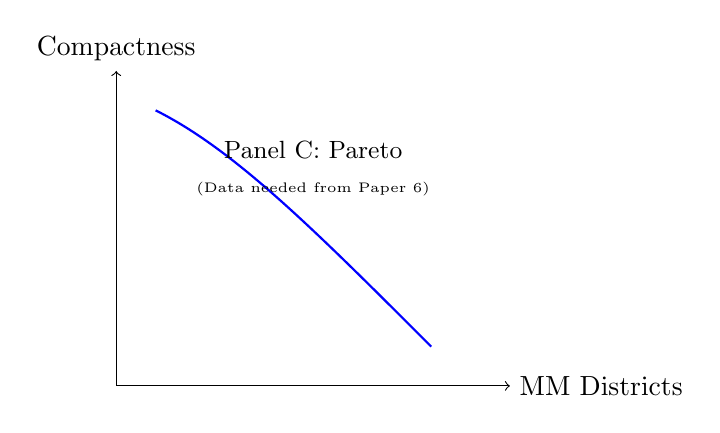
\begin{tikzpicture}[scale=0.5]
% Placeholder - needs actual data
\draw[->] (0,0) -- (10,0) node[right] {MM Districts};
\draw[->] (0,0) -- (0,8) node[above] {Compactness};
% Pareto curve
\draw[thick, blue] (1,7) .. controls (3,6) and (5,4) .. (8,1);
\node at (5,6) {\small Panel C: Pareto};
\node at (5,5) {\tiny (Data needed from Paper 6)};
\end{tikzpicture}
\caption{VRA-compactness tradeoff}
\end{subfigure}

\caption{\textbf{VRA compliance analysis.} (A) Algorithmic plans create 137 majority-minority (MM) districts versus 68 in enacted plans, a surplus of 69 (+101\%). Key states shown: Alabama (0$\rightarrow$2), Georgia (5$\rightarrow$6), Louisiana (1$\rightarrow$2). (B) The 42\% demographic threshold determines where proportional minority representation becomes geographically feasible. States above 42\% minority population achieve near-proportional outcomes; states below 37\% face geometric constraints. (C) Pareto frontier for Alabama shows tradeoff between VRA compliance and geometric compactness, illustrating achievable parameter space.}
\label{fig:vra}
\end{figure*}

% NOTE: This is a placeholder template. Actual figure requires:
% - Data extraction from papers 3, 4, 6
% - Python/R script to generate plots
% - Integration of real state-by-state MM counts
% - Scatter plot data for threshold analysis
% - Pareto frontier coordinates from Alabama case study
